\documentclass[10pt, a4paper]{report}

\usepackage[utf8]{inputenc}
\usepackage{polski}
\usepackage{a4wide}
\usepackage{fancyhdr}
\usepackage{lastpage}
\usepackage{tabularx}
\usepackage{graphicx}
\usepackage{listings}
\usepackage{forest}
\usepackage{xcolor}
\usepackage{epstopdf}


\graphicspath{ {./images} }
\epstopdfDeclareGraphicsRule{.pdf}{png}{.png}{convert #1 \OutputFile}
\DeclareGraphicsExtensions{.png,.pdf}

\definecolor{folderbg}{RGB}{124,166,198}
\definecolor{folderborder}{RGB}{110,144,169}
\definecolor{codegreen}{rgb}{0,0.6,0}
\definecolor{codegray}{rgb}{0.5,0.5,0.5}
\definecolor{codepurple}{rgb}{0.58,0,0.82}
\definecolor{backcolour}{rgb}{0.95,0.95,0.92}

\lstdefinestyle{listings}{
    backgroundcolor=\color{backcolour},   
    commentstyle=\color{codegreen},
    keywordstyle=\color{magenta},
    numberstyle=\tiny\color{codegray},
    stringstyle=\color{codepurple},
    basicstyle=\ttfamily\footnotesize,
    breakatwhitespace=false,         
    breaklines=true,                 
    captionpos=b,
    keepspaces=true,                 
    numbers=left,                    
    numbersep=6pt,                  
    showspaces=false,                
    showstringspaces=false,
    showtabs=false,                  
    tabsize=4
}

\def\Size{4pt}
\tikzset{
  folder/.pic={
    \filldraw[draw=folderborder,top color=folderbg!50,bottom color=folderbg]
      (-1.05*\Size,0.2\Size+5pt) rectangle ++(.75*\Size,-0.2\Size-5pt);  
    \filldraw[draw=folderborder,top color=folderbg!50,bottom color=folderbg]
      (-1.15*\Size,-\Size) rectangle (1.15*\Size,\Size);
  }
}

\begin{titlepage}
    \title{\huge{\textbf{Specyfikacja implementacyjna} \\ programu \textit{"grapher"}}}
    \author{Szymon Półtorak i Sebastian Sikorski}
    \date{28.04.2022r}
\end{titlepage}

\renewcommand{\footrulewidth}{1pt}
\lstset{style=listings}

\begin{document}
    \maketitle
    \renewcommand*\thesection{\arabic{section}}

    \begin{abstract}
      Niniejszy dokument omawia tematykę projekt pod kątem jego implementacji. Tłumaczymy w niej w jaki sposób podeszliśmy do budowy oprogramowania i
      metodykę przeprowadzania testów.
    \end{abstract}

    \pagestyle{fancy}
    \fancyhf{}
    \lhead{Specyfikacja implementacyjna programu \textit{grapher}(Java)}
    \rhead{Szymon Półtorak i Sebastian Sikorski}
    \cfoot{Strona \thepage \hspace{1pt} z \pageref{LastPage}}
    
    \fancypagestyle{plain}{
        \lhead{Specyfikacja implementacyjna programu \textit{grapher}(Java)}
        \rhead{Szymon Półtorak i Sebastian Sikorski}
        \cfoot{Strona \thepage \hspace{1pt} z \pageref{LastPage}}
    }
    \tableofcontents
    \newpage

    \section{Cel Projektu - streszczenie}
    Celem projektu było stworzenie programu mającego za zadanie generowanie grafów, sprawdzanie ich spójności oraz wyszukiwanie w nich najkrótszej ścieżki między zadanymi przez użytkownika punktami. 
    Grafi są typu \textit{kartka w kratkę}.

    \begin{itemize}
        \item Wage Mode – program generuje graf o losowych wagach dróg między wierzchołkami w taki sposób, że jest on spójny,
        \item Edge Mode – program losuje istnienie krawędzi między wierzchołkami grafu oraz wagi do momentu powstania 
        grafu spójnego. Do sprawdzania wykorzystuje algorytm BFS,
        \item Random Mode – program losuje wagi dróg oraz krawędzie między wierzchołkami. W tym trybie graf może być niespójny,
        \item Read Mode -- program odczytuje odpowiednio sformatowany plik i szuka najkrótszej ścieżki
        między podanymi przez użytkownika punktami za pomocą algorytmu Dijkstry.
    \end{itemize}
    Po szczegóły dotyczące tematyki projektu odsyłamy do specyfikacji funkcjonalnej.

    \section{Środowisko powstawania programu}
    Podczas tworzenia programu kluczowe są odpowiednio dobrane narzędzia oraz stałość ich wersji podczas pracy. Narzędzia te prezentujemy w tabeli poniżej:
    \newline \begin{tabularx}{\textwidth}{l|l}
      \hline Nazwa & Wersja \\
      \hline Java & Java SE 17\\
      \hline Java Development Kit & 17.0.3.\\
      \hline Apache Maven & 3.8.5. \\
      \hline InteliJ IDEA & 2021.3.3 \\
      \hline Git & 2.30.2. \\      
      \hline JavaFX & 18.0.1. \\
      \hline
    \end{tabularx}
    \newpage

    \section {Algorytmy}
    Nasz program wykorzystuje dwa algorytmy, które opisujemy w poniższych podrozdziałach.

    \subsection{Algorytm Dijkstry}
    Algorytm Dijkstry liczy najkrótszą odległość od wierzchołka początkowego do wszystkich innych wierzchołków,
    ale w naszej implementacji skupiamy się jedynie na najkrótszej ścieżce między wierzchołkami zadanymi przez
    użytkownika. Algorytm ten korzysta z kopca pełniącego role kolejki priorytetowej oraz trzech tablic przechowujących
    poprzedników, wagi połączeń i i całowity dystans.
    Algorytm dodaje odwiedzane wierchołki do kolejki priorytetowej a nastepnie pobiera je z niej akutalizując dystans
    dopóki kopiec nie jest pusty. Następnie zaczynając od wierzchołka końcowego (podanego przez użytkownika) cofamy się aż trafimy do wierzchołka początkowego.
    Podczas cofania zapisujemy przez jakie wierzchołki przeszliśmy oraz jaka była waga takiego przejścia.
    \begin{figure}[h]
      \begin{center}
          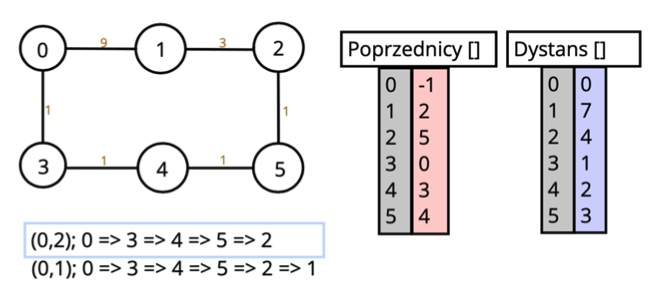
\includegraphics[scale=0.5]{dijkstra.png}
          \caption{Przykładowe działanie algorytmu Dijksty.}
      \end{center}
  \end{figure}
  \newpage

    \subsection{Breadth-first search(BFS)}
    Nasza implementacji algorytmu BFS opiera się na sprawdzaniu tak zwanej "silnej spójności",
    algorytm ten wywoływany jest z każdego wierchołka, rozpoczynając od wierchołka pierwszego.
    Algorytm w celu sprawdzenia spójności tworzy tablicę poprzedników o długości odpowiadającej ilości wierzchołków
    oraz zapełnia ją wartościami -1. Rozpoczynając iteracje od wierzchołka zero aż do ostatniego wierzchołka.
    Algorytm sprawdza z jakimi wierzchołkami połączony jest obecny i dopisuje te wierzchołki do kolejki typu FIFO,
    czyli kolejka typu first in first out, czyli pierwszy wchodzi i wychodzi, jednocześnie uzupełniając tablicę poprzedników.
    Po takim kroku algorytm przechodzi do kolejnego wierzchołka pobierając jego ID z kolejki.
    Przy dotarciu do końca kolejki algorytm musi sprawdzić czy jednym wierzchołkiem bez poprzednika
    jest wierzchołek zero, w przeciwnym przypadku test spójności jest negatywny.

    \begin{figure}[h]
      \begin{center}
          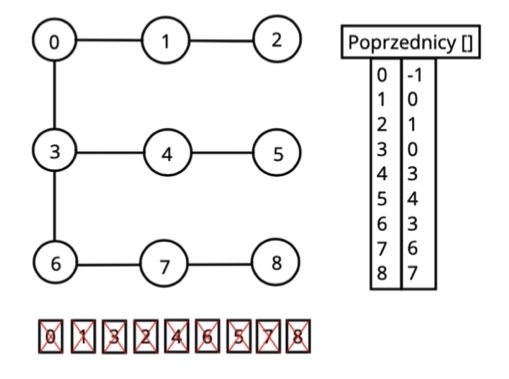
\includegraphics[scale=0.5]{bfs.png}
          \caption{Przykładowe działanie algorytmu BFS.}
      \end{center}
  \end{figure}
  \newpage

  \section{Budowa programu}
  W tym rozdzialne omówimy zagadnienie wzorców projektowych, budowę oraz diagram klas naszego programu.

    \subsection{Wybrany wzorzec projektowy}
    Niniejszy projekt oparty jest na wzorcu projektowym fasady.
    Powoduje to stworzenie jednego prostego interfejsu służącego do sterowania programem
    a jego dodatkową zaletą jest ukrycie przed użytkownikiem złożoności programu.

    \begin{figure}[h]
      \begin{center}
          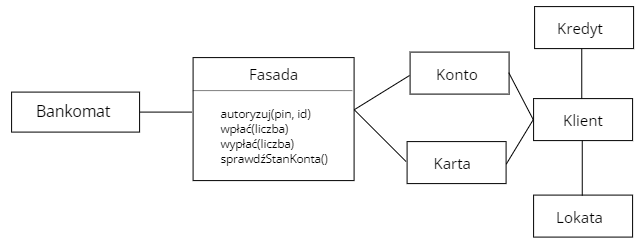
\includegraphics[scale=0.42]{facede.png}
          \caption{Przykładowe zastosowanie fasady na bazie bankomatu.}
      \end{center}
    \end{figure}
    \newpage

    \subsection{Wykorzystane klasy}
    Poniższa lista zawiera klasy wykorzystane w programie. Ich powiązania widoczne są na diagramie klas w następnym podrozdzialne.

    \begin{itemize}
      \item \texttt{GrapherClient} -- odpowiedzialna za interakcje z użytkownikiem,
      \item \texttt{GrapherControler} -- klasa będąca fasadą, ukrywa złożoność aplikacji przed użytkownikiem,
      \item \texttt{EntryData} -- klasa odpowiedzialna za przechowywanie informacji wprowadzonych przez użytkownika,
      \item \texttt{Graph} -- klasa przechowująca graf,
      \item \texttt{Vertex} -- klasa przechowująca wierchołek oraz informacje na temat krawędzi wychodzących z danego wierchołka,
      \item \texttt{Existence} -- klasa przechowująca informacje o tym, czy istnieje połaczenie z danego wierchołka w danym kierunku,
      \item \texttt{Weights} -- klasa przechowująca informacje o wagach połączeń między punktami,
      \item \texttt{Connect} -- klasa przechowująca informacje o tym dokąd prowadzi dane połączenia,
      \item \texttt{GraphIO} -- klasa odpowiedzialna za obsługę plików,
      \item \texttt{GraphGenerator} -- klasa odpowiedzialna za generację grafu,
      \item \texttt{WageMode} -- klasa odpowiedzialna za tryb wag,
      \item \texttt{EdgeMode} -- klasa odpowiedzialna za tryb krawędzi,
      \item \texttt{RandomMode} -- klasa odpowiedzialna za tryb losowy,
      \item \texttt{Dijkstra} -- klasa odpowiedzialna za wyszukiwanie najkrótszej ścieżki,
      \item \texttt{PathPrinter} -- klasa odpowiedzilna za wyświetlanie obliczonej już najkrótszej ścieżki,
      \item \texttt{BFS} -- klasa odpowiedzialna za sprawdzanie spójności grafu,
      \item \texttt{Heap} -- klasa odpowiedzialna za kolejkę priorytetą w postaci kopca,
      \item \texttt{PathData} -- klasa odpowiedzialna za przechowywanie informacji klucziowych dla wyszukiwania najkrótszej ścieżki.
    \end{itemize}
    \newpage

    \subsection{Diagram klas}
    Dokładne powiązania między klasami reprezentuje poniższy diagram. Zawiera on tylko najważniejsze metody każdej klasy.
    \begin{figure}[h]
        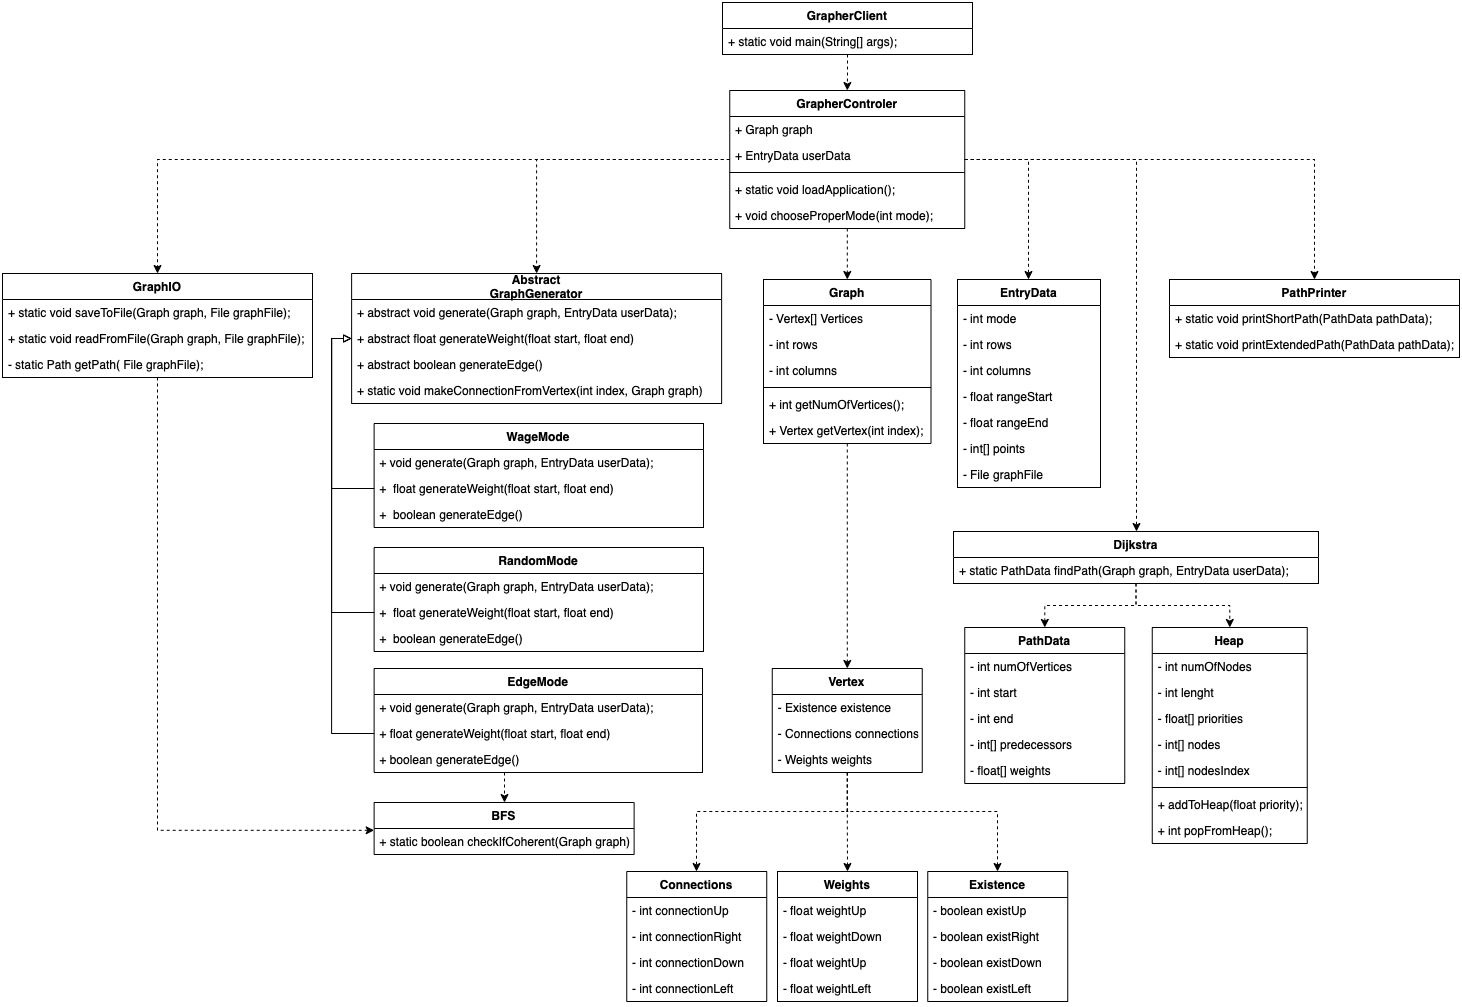
\includegraphics[scale=0.29]{ClassDiagram.png}
        \caption{Diagram klas.}
  \end{figure}
  \newpage

    \section{Testowanie programu}
    Testowanie jednostkowe programu będzie przeprowadzone z wykorzystaniem framework'u JUnit oraz biblioteki AssertJ.
    Testowane będą najważniejsze funkcjonalności programu oraz poszczególne interakcje między nimi. 
    Testom poddana będzie także umiejętność rozpoznawania przez program niepoprawnych danych wejściowcyh tak 
    aby program zachowywał się zgodnie z implementacją funkcjonalną.

    \section{Wprowadzanie zmian}
    Zmiany wprowadzane były za pomocą systemu kontroli \texttt{Git}. Poszczególne zadania były wykonywane za pomocą osobnych gałęzi (branchy), a zmiany wprowadzane
     za pomocą commitów. Złączanie gałęzi z główną \textit{masterem} było przeprowadzane po akcpetacji kodu przez drugiego członka zespołu.

    \section{Konwencje nazewnicze}
    W celu utrzymania czytelności i przejrzystości kodu przyjęliśmy niniejsze konwencje nazewnicze:
    \begin{itemize}
      \item Wszystkie nazwy i komunikaty w języku angielskim,
      \item Wszelkie instrukcje wewnątrz instrukcji \texttt{if} i wszystkich pętli muszą być wewnątrz nawiasów klamrowych,
      \item Adnotacje znajdują się zawsze w wierszu poprzedzającym metodą, do której się odnoszą,
      \item Nazwy zmiennych i klas są pisane w konwencji CamelCase. Zmienne zaczynam małą literą i rozpoczęcie drugiego słowa zaczyna się wielką literą, czyli słowo "is empty" jako zmienna i metoda to "isEmpty", a klasa
      "IsEmpty".
    \end{itemize}

\end{document}